\chapter{Informatyka afektywna}
\label{cha:affectiveComputing}

Informatyka afektywna (ang. \textit{affective computing}) jest dziedziną informatyki, w~której obliczenia są powiązane z~emocjami lub bezpośrednio na nie wpływają~\cite{Picard:1997:AC:265013}. Głównym celem informatyki afektywnej jest rozpoznawanie oraz analiza emocji ludzkich, możliwość ich symulacji przez komputer, a także wpływanie na emocje użytkownika poprzez konkretne bodźce. Aby uzyskać taki efekt, informatyka afektywna jest silnie powiązana z~dziedzinami takimi jak psychologia, fizjologia, czy kognitywistyka~\cite{affective_computing_review_tao_tieniu}.

\section{Emocje}
Choć do dzisiaj nie ma jednej, uniwersalnej definicji czym są emocje, to środowisko naukowe ciągle przeprowadza badania na tematy powiązane z~emocjami. Już w~XIX wieku powstała teoria opracowana niezależnie przez Williama Jamesa oraz Carla Lange'a, gdzie emocję zdefiniowano jako interpretację reakcji cielesnej na zaobserwowany bodziec~\cite{Coleman2011}. Obaj badacze przyjęli, że na konkretny czynnik człowiek reaguje najpierw reakcją fizjologiczną. Następnie zostaje ona przez niego przypisana do wzorca odpowiadającego danej emocji. Dla przykładu, jeśli człowiek znajdzie się w~sytuacji, w~której zobaczy zagrożenie, zaczyna się trząść i~pocić. Jednocześnie jego tętno gwałtownie wzrasta, mózg natomiast interpretuje to jako strach.

Teoria Jamesa-Lange'a została zakwestionowana w~latach dwudziestych XX wieku przez dwójkę naukowców, Waltera Cannona i~Phillipa Barda. Zasugerowali oni, że odczuwanie emocji nie jest zależne od reakcji fizjologicznych, a raczej są to reakcje zachodzące jednocześnie jako odpowiedź na dany bodziec~\cite{cannon_1927}. Koncepcja ta była bezpośrednim zakwestionowaniem badań przeprowadzonych przez Jamesa i~Lange'a. Jej autorzy przeprowadzili badania na kotach, na podstawie których przedstawili, iż to wzgórze jest obszarem mózgu odpowiedzialnym za reakcje emocjonalne na doświadczane bodźce. Cannon zauważył, że całkowite odcięcie wszystkich układów od mózgu nie zmienia zachowania emocjonalnego zwierząt, co kłóciło się z~teorią Jamesa-Lange'a, według której koty powinny przestać wykazywać jakiekolwiek reakcje emocjonalne.

\begin{figure}[h]
	\centering
	\begin{subfigure}{0.7\textwidth}
		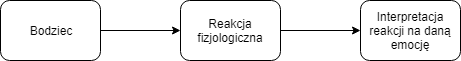
\includegraphics[width=\linewidth]{images/james-lang.png}
		\label{fig:james}
		\caption{Teoria Jamesa-Lange'a, źródło: opracowanie własne na podstawie~\cite{Coleman2011}}
	\end{subfigure}
	\begin{subfigure}{0.7\textwidth}
		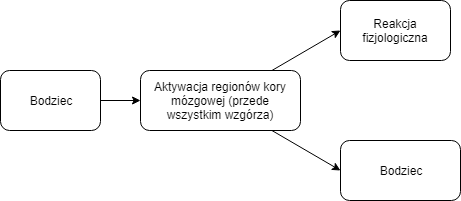
\includegraphics[width=\linewidth]{images/cannon-bard.png}
		\label{fig:canon}
		\caption{Teoria Canona-Barda, źródło: opracowanie własne na podstawie~\cite{cannon_1927}}
	\end{subfigure}
	\caption{Graficzne porównanie teorii emocji Jamesa-Lange'a i~Canona-Barda}
\end{figure}

Teoria Jamesa-Lange'a została ponownie podjęta przez Prinza, który przedstawił więcej dowodów na potwierdzenie tej teorii, jednocześnie opisując argumenty pokazujące, że reakcje fizjologiczne nie zawsze są wystarczające lub w~ogóle niepotrzebne do odczuwania emocji~\cite{Prinz2004-PRIEE-2}. Zwrócił on między innymi uwagę na badania Hohmanna nad pacjentami z~urazami rdzenia kręgowego~\cite{Hohmann1966SomeEO}, w~których zauważono efekty zarówno potwierdzające, jak i~podające w~wątpliwość teorię Jamesa-Lange'a. Hohmann zaobserwował, że u osób z~urazem można dostrzec redukcję w~odczuwaniu emocji, ale niektóre z~nich wciąż były widoczne. Prinz komentuje to jako zdolność mózgu do przewidzenia reakcji fizjologicznej na dany bodziec, co z~kolei będzie skutkować odczuwaniem emocji. Jest to możliwe dzięki wcześniejszym doświadczeniom. Tak jak człowiek tracący wzrok, jest w~stanie wyobrazić sobie przedmiot, który kiedyś widział, tak samo mózg potrafi określić jaka reakcja fizjologiczna mogła nastąpić na dany bodziec.

\section{Modele emocji}
Ponieważ emocje są pojęciem abstrakcyjnym, ich pomiar oraz analiza w~informatyce afektywnej nie jest prosta i~wymaga przyjętego modelu pozwalającego na jednoznaczny pomiar emocji. Na przestrzeni lat powstało wiele modeli opisujących emocje, które można podzielić na dwa główne typy~\cite{emotion_models_review_2017}:
\begin{itemize}
	\item modele kategoryzowane, w~których określony jest zbiór emocji reprezentowanych przez konkretne oznaczenia
	\item modele wymiarowe, w~których emocje są reprezentowane przy pomocy zbioru miar określających ich własności.
\end{itemize}

\subsection{Modele kategoryzowane}
Do typu modeli kategoryzowanych zaliczają się przede wszystkim modele emocji bazowych. Na przestrzeni lat powstało wiele modeli różniących się od siebie ilością oraz rodzajami emocji. Przykładem może być tutaj model zaproponowany przez Oatley'a i~Johnsona-Lairda, w~którym proponują oni pięć podstawowych emocji: gniew, lęk, odraza, radość i~smutek~\cite{oatley_theory_of_emotions}. Jednym z~popularniejszych modeli emocji bazowych, jest ten przedstawiony przez Ekmana. Razem z~Friesenem przeprowadzili badania na plemieniu z~Papui Nowej Gwinei. Członkowie plemienia byli w~stanie zidentyfikować sześć emocji: strach, gniew, wstręt, smutek, szczęście i~zaskoczenie (rys. \ref{fig:ekman_six_emotions})~\cite{Ekman1971ConstantsAC}. Kilka lat później do tej grupy Ekman dodał pogardę, aby odróżnić ją od wstrętu. 
\begin{figure}[h]
	\centering
	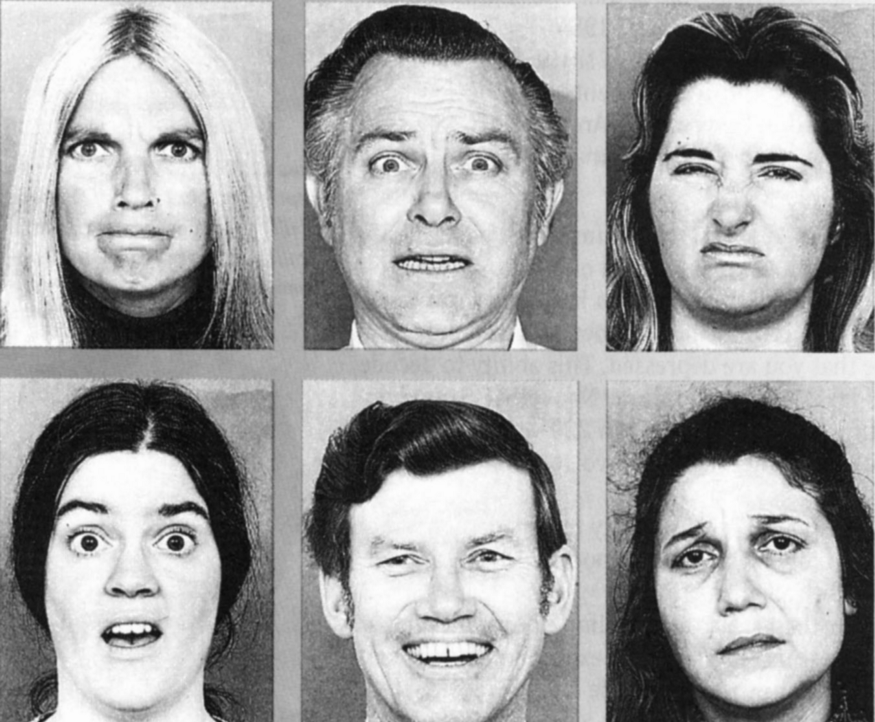
\includegraphics[width=0.6\linewidth]{images/ekman_six_basic_emotions.png}
	\caption{Wyrazy twarzy odpowiadające sześciu emocjom zaproponowanym przez Ekmana, źródło: \cite{Ekman1971ConstantsAC}}
	\label{fig:ekman_six_emotions}
\end{figure}

W modelach kategoryzowanych, często nazywanych także modelami dyskretnymi, emocje są niezależne od siebie. Ich dużą zaletą jest to, że automatycznie reprezentują ludzkie emocje dzięki łatwym do zrozumienia etykietom. Jednak w~swojej pracy James Russell i~Lisa Barret przedstawiają problemy, jakie można napotkać w~tym typie modeli~\cite{russel_barret_core_affect}. Pierwszym są różnice występujące w~nazwach kategorii w~zależności od języka. Każdy ze stanów emocjonalnych może być opisany na różne sposoby w~zależności od języka. Różnice mogą wystąpić nie tylko w~samym tłumaczeniu, ale nawet w~ilości słów opisujących daną emocję. Kolejnym problemem jest fakt, że granice pomiędzy danymi klasami emocji często są rozmyte. Te same stany emocjonalne można wyrazić za pomocą różnych kategorii w~zależności od różnic kulturowych, środowiskowych czy osobowościowych~\cite{emotion_models_review_2017}. Trzecim przedstawionym problemem jest to, że każdy z~typów emocji, takich jak gniew czy strach, składa się z~zestawu uporządkowanych w~czasie powiązanych ze sobą zdarzeń. W~związku z~tym takie emocje powinno traktować jako złożone procesy, które nie powinny być traktowane jako elementy atomowe.

\subsection{Modele wymiarowe}

Russell w~swoich badaniach zauważył jeszcze jeden istotny problem modeli dyskretnych. Skoro opisują one stany emocjonalne w~sposób jednoznaczny, nie można określić poziomu odczuwania emocji. Jako przykład podaje porównanie strachu w~trakcie przejażdżki kolejką górską a sytuacjami zagrażającymi życiu. W~przypadku modeli dyskretnych w~obu sytuacjach można jedynie określić odczuwanie emocji strachu, pomimo różniących się reakcji fizjologicznych. W~ramach swoich badań Russel zaproponował model w~kształcie okręgu, składający się z~dwóch wymiarów (rys. \ref{fig:circumplex}). Pierwszym z~nich jest poziom odczuwania przyjemności w~modelu nazwany wartościowością (ang. \textit{valence}). Odzwierciedlał on także pozytywność lub negatywność emocji. Niskie wartości odpowiadają emocjom takim jak smutek, stres, czy odraza, natomiast szczęście lub ekscytacja są opisane poprzez wysokie wartości wartościowości. Drugim wymiarem jest pobudzenie (ang. \textit{arousal}), które opisuje natężenie danej emocji. Odczucia takie jak senność, depresja czy zrelaksowanie charakteryzują się niskimi wartościami pobudzenia, natomiast wartościom wysokim odpowiadają emocje takie jak ekscytacja, zaskoczenie, czy złość. Model został przedstawiony w~formie koła, na którego brzegach opisane zostały podstawowe emocje. Warto wspomnieć, że nie jest to pierwszy model o strukturze kołowej. Sam Russel, chcąc pokazać uniwersalność swojego modelu, porównuje go między innymi z~teoriami zaproponowanymi przez Watsona i~Tellegena~\cite{Watson_1985}. Tym, co wyróżniało model Russela, były przeprowadzone badania~\cite{circumplex_model_russel_1980}. Russel wybrał 28 słów reprezentujących konkretne stany afektywne i~przy pomocy trzech różnych technik przeskalował je, otrzymując zbliżone wyniki. W celu potwierdzenia swojej teorii przeprowadził eksperyment z~grupą 36 osób, która miała przyporządkować wybrane słowa do ośmiu kategorii określających podstawowe stany emocjonalne, a następnie ułożyć te kategorie na modelu kołowym w~taki sposób, aby przeciwne emocje znalazły się po przeciwnych stronach koła.

\begin{figure}[h]
	\centering
	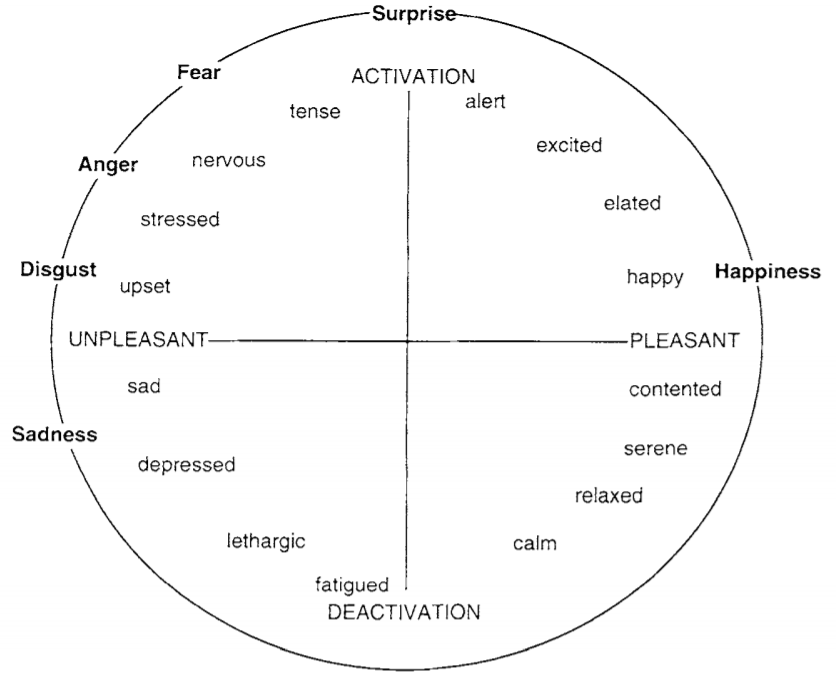
\includegraphics[width=0.6\linewidth]{images/circumplex.png}
	\caption{Model wymiarowy zaproponowany przez Russela, źródło: \cite{russel_barret_core_affect}}
	\label{fig:circumplex}
\end{figure}

Kilka lat później Russel wraz z~Anną Weiss oraz Geraldem Mendelsohnem przedstawił propozycję jednopunktowej skali nazwaną Affect Grid, która miała służyć jako sposób szybkiej i~prostej do analizy oceny stanów afektywnych wzdłuż wymiarów znanych z~modelu Russela, wartościowości oraz pobudzenia~\cite{affect_grid_russel_1989}. Skala jest przedstawiona w~formie siatki, gdzie oba wymiary określane są w~zakresach od 1 do 9 w~sposób ciągły. Początkowo miała ona mieć formę kołową, podobną do kołowej struktury modeli emocji, jednak ostatecznie zrezygnowano z~niej na rzecz znacznie prostszej do wytłumaczenia badanym osobom siatki. W~ramach sprawdzenia, czy przedstawiona skala w~poprawny sposób odzwierciedla stany emocjonalne, przeprowadzono badania, w~których wykorzystano między innymi słowa wybrane przy wcześniejszych badaniach Russela oraz zbiór zdjęć z~wyrazami twarzy odpowiadającymi konkretnym stanom afektywnym. Zadaniem badanych było oznaczenie na skali poziomu wartościowości i~pobudzenia najlepiej odzwierciedlających dane słowo lub wyraz twarzy. Następnie wyniki porównano z~innymi skalami opisującymi poziomy wartościowości i~zauważono wysoki stopień podobieństwa między nimi. 

\begin{figure}[h]
	\centering
	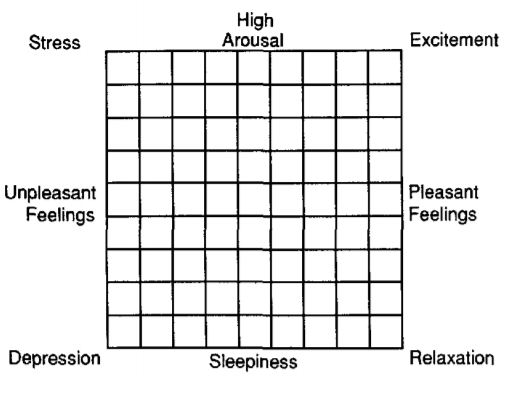
\includegraphics[width=0.5\linewidth]{images/affect_grid.png}
	\caption{\textit{Affect Grid}, źródło:~\cite{affect_grid_russel_1989}}
	\label{fig:affect_grid}
\end{figure}

Model emocji przedstawiony przez Russela oraz skala opisana w~\textit{Affect Grid} stały się jednymi z~bardziej popularnych form przedstawiania emocji w~informatyce afektywnej. Ogromną ich zaletą jest przede wszystkim łatwość przetwarzania danych opartych na dwuwymiarowej skali, które określają dane stany emocjonalne. Skalę tą można zauważyć między innymi w~zbiorach danych zawierających powiązania między reakcjami fizjologicznymi a odpowiednimi wartościami wartościowości i~pobudzenia~\cite{deap_dataset_2011,amigos_dataset_2017}. 

\section{Pętla afektywna}
Do realizacji celów zakładanych przez informatykę afektywną~\cite{Picard:1997:AC:265013} wykorzystywana jest pętla afektywna. To pochodzące z~dziedziny Automatyki i~Robotyki pojęcie zakłada, że system oraz środowisko są zaangażowane w~ciągłą interakcję między sobą. Schemat pętli został przedstawiony na rysunku~\ref{fig:affective_loop}.\newpage Kristina Höök przedstawiła definicję pętli afektywnej w~formie trzech kroków~\cite{affective_loop_experiences}:
\begin{enumerate}
	\item Użytkownicy wyrażają emocje poprzez pewne  interakcje obejmujące ich ciało, na przykład gesty czy inne akcje wpływające na środowisko.
	\item Następnie odpowiada środowisko generujące elementy afektywne, używając na przykład kolorów, animacji czy innej formy, która może wpłynąć na użytkowników.
	\item Elementy afektywne wpływają na reakcję użytkowniów, co prowadzi do coraz większego ich zaangażowania w~interakcję ze środowiskiem.
\end{enumerate}

Jak widać, istotnym elementem pętli jest sposób określenia stanów emocjonalnych danej osoby. Spoglądając na rozwiązania praktyczne, można zauważyć, że duże znaczenie ma wykorzystanie sztucznej inteligencji do przewidywania emocji na podstawie reakcji fizjologicznych~\cite{emotional_context_geist_2019}. Wykorzystywane są tutaj przede wszystkim wcześniej opisane modele Ekmana~\cite{Ekman1971ConstantsAC} oraz Russela~\cite{circumplex_model_russel_1980}, które przedstawiają emocję w~formie zrozumiałej dla komputera. Same emocje są natomiast przewidywane na podstawie odczytów reakcji fizjologicznych użytkowników, a także ich interakcji ze środowiskiem. Określenie stanu emocjonalnego użytkownika pozwala na generację w~środowisku sytuacji, które wpłyną na użytkownika tak, aby ten mógł zareagować w~odpowiedni sposób i~zwiększać swoje zaangażowanie w~interakcję ze środowiskiem. 

Dobrym przykładem systemów wykorzystujących pętlę afektywną są systemy świadome kontekstu, takie jak afektywne odtwarzacze muzyki~\cite{Janssen2012,ChrzanowskaInzynierska}, które na podstawie sygnałów odczytanych od użytkownika modyfikują listę odtwarzanych piosenek, tak, aby dopasować ją do aktualnego stanu emocjonalnego użytkownika i~w~wybrany sposób na niego wpłynąć.

\begin{figure}
	\centering
	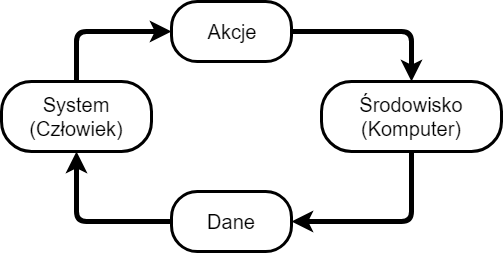
\includegraphics[width=0.6\linewidth]{images/affective_loop.png}
	\caption{Cykl pętli afektywnej, źródło: opracowanie własne na podstawie~\cite{affective_loop_experiences}}
	\label{fig:affective_loop}
\end{figure}

\section{Gry z~pętlą afektywną}
W ciągu ostatnich lat znacznie wzrosło zainteresowanie grami komputerowymi zawierającymi elementy informatyki afektywnej. Głównym celem tworzenia gier jest dostarczenie użytkownikowi rozrywki poprzez zwiększanie poziomu immersji~\cite{jennet_immersion_in_games_2008}, często również dzięki zapewnieniu wrażeń emocjonalnych. Końcowy odbiór zależny jest między innymi od takich elementów jak fabuła, mechaniki wykorzystane w~trakcie rozgrywki, czy też szczegóły wizualne. Aby jak najlepiej zadowolić użytkownika, twórcy gier muszą także wykorzystywać najnowsze technologie, które mogą sprawić, że gracz będzie w~stanie jeszcze mocniej odczuwać wrażenia płynące z~rozgrywki. 

Jednym z~takich rozwiązań jest właśnie informatyka afektywna i~wykorzystanie emocji do zwiększenia możliwości wpływania na grę. Eva Hudlicka w~swoich pracach~\cite{hudlicka_2008} wskazuje na kluczowe znaczenie emocji w~projektowaniu gry. Wywołanie ich u gracza jest możliwe dzięki istotnym momentom w~fabule gry, interakcji z~postaciami, do których użytkownik może się w~pewien sposób odnieść emocjonalnie, czy nawet poprzez same mechaniki zaimplementowane w~grze. Ten sam efekt można także uzyskać przez wygląd środowiska, w~którym zostaje umieszczony gracz. Odpowiednie nacechowanie wykorzystanych kolorów, dźwięki otoczenia, czy budowa miejsca, gdzie znajduje się postać prowadzona przez gracza, mogą wpłynąć na to, jakie emocje odczuwa gracz. Idealnym przykładem są tutaj modyfikacje graficzne takich tytułów jak Minecraft czy The Elder Scrolls V: Skyrim. Zapewniają one tekstury wyższej jakości, zbliżone jak najbardziej do tego, co gracz może zobaczyć za oknem w~realnym świecie. Pozwala to na zwiększenie immersji poprzez dostarczanie graczowi doświadczeń zbliżonych do rzeczywistości.

Powyższy sposób wpływania na emocje Hudlicka nazywa otwartą pętlą. W~tym podejściu nie jest wymagane badanie reakcji gracza. Głównym celem jest wpłynięcie na emocje przy pomocy elementów świata gry. Istnieje wiele rozwiązań komercyjnych, które, choć wprost nie są nazywane grami afektywnymi, realizują opisane wyżej założenia. Doskonałym przykładem są tutaj gry przygodowe od studia Telltale Games, gdzie rozgrywka jest formą interaktywnego filmu. W~trakcie rozgrywki gracz podejmuje kluczowe decyzje (rys. \ref{fig:walking_dead}) wpływające na to, jak potoczy się dalsza fabuła gry. Taka forma przedstawienia historii pozwala na zaangażowanie gracza w~poznanie postaci i~przywiązanie się do nich~\cite{games_for_empathy}. Dzięki temu, w~kluczowych momentach, takich jak na przykład odejście czy śmierć bohatera, w~graczu mogą zostać wywołane adekwatne do wydarzenia emocje.
\begin{figure}
	\centering
	
\includegraphics[width=0.7\linewidth]{images/walking_dead_decision.jpg}
	\caption{Przykład kluczowej decyzji w~grze The Walking Dead, źródło:~\cite{the_walking_dead}}
	\label{fig:walking_dead}
\end{figure}

Drugim sposobem jest wykorzystanie odczuwanych przez gracza emocji do modyfikacji systemów zaimplementowanych w~grze tak, aby dostosować je do potrzeb użytkownika i~utrzymać jego zaangażowanie. Przykładem zamkniętej pętli, jak nazywana jest ta metoda przez Hudlicką, jest zmiana stopnia trudności na podstawie samopoczucia gracza. Jeżeli jest on zdenerwowany czy przestraszony, poziom skomplikowania rozgrywki zmniejsza się, natomiast gdy zaczyna on odczuwać nudę, stawiane są przed nim nowe wyzwania, które wzbudzą jego zainteresowanie grą. Zamknięta pętla może być także wykorzystywana w~kontekście gier poważnych. Dla przykładu gry wykorzystywane w~terapiach mogą na bieżąco monitorować stan emocjonalny użytkownika i~modyfikować rozgrywkę w~taki sposób, aby osiągnąć konkretny rodzaj emocji.

Ważnym aspektem, na który należy zwrócić uwagę, jest odpowiednie dobranie elementów sprzętowych wykorzystanych do określenia stanu emocjonalnego użytkownika. Ponieważ środowisko odbiorców gier komputerowych wykracza daleko poza aspekty naukowe, istotne jest to, aby urządzenia nie przeszkadzały w~rozgrywce, a jednocześnie pozwalały na dokładne określenie, jakie emocje odczuwa gracz. W~kolejnych rozdziałach niniejszej pracy omówiono przykłady takich urządzeń, wraz z~ich zaletami i~wadami w~kontekście odczytywania emocji, oraz przystępności dla graczy poza warunkami laboratoryjnymi.

Choć świadome wykorzystanie gier afektywnych jest bardziej widoczne w~środowisku naukowym i~akademickim~\cite{affective_design_patterns_2017,prototypes_affective_games_2019}, to producenci gier starają się powoli wprowadzać kontekst emocjonalny w~komercyjnych rozwiązaniach jako dodatkowy element urozmaicający rozgrywkę~\cite{nevermind_gamesradar,bring_to_light_steam}. Jednym z~głównych problemów jest niewielka ilość opracowań, w~których omówione by zostały dostępne rozwiązania sprzętowe umożliwiające predykcję emocji, oraz to, w~jaki sposób zaimplementować odczytywanie i~reakcje na stany emocjonalne w~środowiskach do tworzenia gier. Z~tego właśnie powodu powstała idea opracowania platformy, która w~prosty sposób może zostać wcielona do istniejącej już gry stworzonej w~określonym oprogramowaniu do tworzenia gier.